\documentclass[10.5pt]{article}

\usepackage{fancyhdr,graphicx,multicol,paralist,times,url,wrapfig,xspace}

\setcounter{page}{1}

\setlength{\textwidth}{7.35in}
\setlength{\textheight}{9.6in}
\setlength{\topmargin}{-0.85in}
\setlength{\oddsidemargin}{-0.38in}

\thispagestyle{plain}
\pagestyle{fancy}
\lhead{}
\rhead{Meng Jiang -- Research Statement}
\cfoot{\thepage}

\makeatletter
\renewenvironment{thebibliography}[1]
     {\begin{multicols}{2}[\section*{{\normalsize REFERENCES}\vskip -0.15in}]%
      \@mkboth{\MakeUppercase\refname}{\MakeUppercase\refname}%
      \list{\@biblabel{\@arabic\c@enumiv}}%
           {\settowidth\labelwidth{\@biblabel{#1}}%
            \leftmargin\labelwidth
            \advance\leftmargin\labelsep
            \@openbib@code
            \usecounter{enumiv}%
            \let\p@enumiv\@empty
            \renewcommand\theenumiv{\@arabic\c@enumiv}}%
      \sloppy
      \clubpenalty4000
      \@clubpenalty \clubpenalty
      \widowpenalty4000%
      \sfcode`\.\@m}
     {\def\@noitemerr
       {\@latex@warning{Empty `thebibliography' environment}}%
      \endlist\end{multicols}}
\makeatother

\newcommand{\lb}{\mbox{$\langle$}}
\newcommand{\rb}{\mbox{$\rangle$}}
\newcommand{\pair}[2]{{\lb#1, #2\rb}\xspace}
\newcommand{\tuple}[3]{{\lb#1, #2, #3\rb}\xspace}
\newcommand{\eapatterns}{{``$E$-$A$'' patterns}\xspace}
\newcommand{\saopatterns}{{``$S$-$A$-$O$'' patterns}\xspace}

\begin{document}

\newcommand{\scxdocument}{$\mathcal{D}$\xspace}
\newcommand{\scxword}{$w$\xspace}
\newcommand{\scxphrase}{$p$\xspace}
\newcommand{\scxmark}{$m$\xspace}
\newcommand{\scxwordset}{$\mathcal{W}$\xspace}
\newcommand{\scxphraseset}{$\mathcal{P}$\xspace}
\newcommand{\scxmarkset}{$\mathcal{M}$\xspace}
\newcommand{\scxentity}{$e$\xspace}
\newcommand{\scxname}{$a$\xspace}
\newcommand{\scxvalue}{${v}_{i}$\xspace}
\newcommand{\scxvaluearray}{$\mathbf{v}$\xspace}
\newcommand{\scxclass}{\textsc{C}\xspace}
\newcommand{\scxnameset}{$\mathcal{A}$\xspace}
\newcommand{\scxvaluetype}{${T}_{i}$\xspace}
\newcommand{\scxvaluetypearray}{$\mathbf{T}$\xspace}
\newcommand{\scxentityset}{$\mathcal{E}$\xspace}
\newcommand{\scxallentityset}{$\mathcal{E}^{+}$\xspace}
\newcommand{\scxclassset}{$\mathcal{C}$\xspace}
\newcommand{\scxallclassset}{$\mathcal{C}^{+}$\xspace}
\newcommand{\scxhierarchy}{$\mathcal{H}$\xspace}
\newcommand{\scxmetapattern}{$MP$\xspace}

\newcommand{\scdocument}{$\mathcal{D}$}
\newcommand{\scword}{$w$}
\newcommand{\scphrase}{$p$}
\newcommand{\scmark}{$m$}
\newcommand{\scwordset}{$\mathcal{W}$}
\newcommand{\scphraseset}{$\mathcal{P}$}
\newcommand{\scmarkset}{$\mathcal{M}$}
\newcommand{\scentity}{$e$}
\newcommand{\scname}{$a$}
\newcommand{\scvalue}{${v}_{i}$}
\newcommand{\scvaluearray}{$\mathbf{v}$}
\newcommand{\scclass}{\textsc{C}}
\newcommand{\scnameset}{$\mathcal{A}$}
\newcommand{\scvaluetype}{${T}_{i}$}
\newcommand{\scvaluetypearray}{$\mathbf{T}$}
\newcommand{\scentityset}{$\mathcal{E}$}
\newcommand{\scallentityset}{$\mathcal{E}^{+}$}
\newcommand{\scclassset}{$\mathcal{C}$}
\newcommand{\scallclassset}{$\mathcal{C}^{+}$}
\newcommand{\schierarchy}{$\mathcal{H}$}
\newcommand{\scmetapattern}{$MP$}

\newcommand{\cslocation}{$\$$\textsc{Location}\xspace}
\newcommand{\csaqua}{$\$$\textsc{Aqua}\xspace}
\newcommand{\csocean}{$\$$\textsc{Ocean}\xspace}
\newcommand{\csriver}{$\$$\textsc{River}\xspace}
\newcommand{\cssea}{$\$$\textsc{Sea}\xspace}
\newcommand{\csgovloc}{$\$$\textsc{GovLoc}\xspace}
\newcommand{\cscity}{$\$$\textsc{City}\xspace}
\newcommand{\cscnprovince}{$\$$\textsc{CNProvince}\xspace}
\newcommand{\cscountry}{$\$$\textsc{Country}\xspace}
\newcommand{\cscounty}{$\$$\textsc{County}\xspace}
\newcommand{\csethnicity}{$\$$\textsc{Ethnicity}\xspace}
\newcommand{\csusstate}{$\$$\textsc{USState}\xspace}
\newcommand{\csland}{$\$$\textsc{Land}\xspace}
\newcommand{\csisland}{$\$$\textsc{Island}\xspace}
\newcommand{\cspeninsula}{$\$$\textsc{Peninsula}\xspace}
\newcommand{\cspath}{$\$$\textsc{Path}\xspace}
\newcommand{\csavenue}{$\$$\textsc{Avenue}\xspace}
\newcommand{\csboulevard}{$\$$\textsc{Boulevard}\xspace}
\newcommand{\csdrive}{$\$$\textsc{Drive}\xspace}
\newcommand{\csroad}{$\$$\textsc{Road}\xspace}
\newcommand{\csstreet}{$\$$\textsc{Street}\xspace}
\newcommand{\cspoi}{$\$$\textsc{POI}\xspace}
\newcommand{\csairport}{$\$$\textsc{Airport}\xspace}
\newcommand{\csbridge}{$\$$\textsc{Bridge}\xspace}
\newcommand{\cshospital}{$\$$\textsc{Hospital}\xspace}
\newcommand{\cssquare}{$\$$\textsc{Square}\xspace}
\newcommand{\csstadium}{$\$$\textsc{Stadium}\xspace}
\newcommand{\csstation}{$\$$\textsc{Station}\xspace}
\newcommand{\csorganization}{$\$$\textsc{Organization}\xspace}
\newcommand{\cscompany}{$\$$\textsc{Company}\xspace}
\newcommand{\csairlines}{$\$$\textsc{Airlines}\xspace}
\newcommand{\csevent}{$\$$\textsc{Event}\xspace}
\newcommand{\csattack}{$\$$\textsc{Attack}\xspace}
\newcommand{\csaward}{$\$$\textsc{Award}\xspace}
\newcommand{\csfestival}{$\$$\textsc{Festival}\xspace}
\newcommand{\cssummit}{$\$$\textsc{Summit}\xspace}
\newcommand{\csgame}{$\$$\textsc{Game}\xspace}
\newcommand{\cspolicy}{$\$$\textsc{Policy}\xspace}
\newcommand{\csprotest}{$\$$\textsc{Protest}\xspace}
\newcommand{\cswar}{$\$$\textsc{War}\xspace}
\newcommand{\csgovernment}{$\$$\textsc{Government}\xspace}
\newcommand{\csinstitute}{$\$$\textsc{Institute}\xspace}
\newcommand{\csinternational}{$\$$\textsc{International}\xspace}
\newcommand{\csmilitantgroup}{$\$$\textsc{MilitantGroup}\xspace}
\newcommand{\csmovie}{$\$$\textsc{Movie}\xspace}
\newcommand{\csnewsagency}{$\$$\textsc{NewsAgency}\xspace}
\newcommand{\csparty}{$\$$\textsc{Party}\xspace}
\newcommand{\csproduct}{$\$$\textsc{Product}\xspace}
\newcommand{\csreligion}{$\$$\textsc{Religion}\xspace}
\newcommand{\cssportsleague}{$\$$\textsc{SportsLeague}\xspace}
\newcommand{\cssportsteam}{$\$$\textsc{SportsTeam}\xspace}
\newcommand{\csteamname}{$\$$\textsc{TeamName}\xspace}
\newcommand{\csperson}{$\$$\textsc{Person}\xspace}
\newcommand{\csartist}{$\$$\textsc{Artist}\xspace}
\newcommand{\csactor}{$\$$\textsc{Actor}\xspace}
\newcommand{\csauthor}{$\$$\textsc{Author}\xspace}
\newcommand{\csdirector}{$\$$\textsc{Director}\xspace}
\newcommand{\csmodel}{$\$$\textsc{Model}\xspace}
\newcommand{\cssinger}{$\$$\textsc{Singer}\xspace}
\newcommand{\cstvhost}{$\$$\textsc{TVHost}\xspace}
\newcommand{\cstvpersonality}{$\$$\textsc{TVPersonality}\xspace}
\newcommand{\csathlete}{$\$$\textsc{Athlete}\xspace}
\newcommand{\csbaseballplayer}{$\$$\textsc{BaseballPlayer}\xspace}
\newcommand{\csbasketballplayer}{$\$$\textsc{BasketballPlayer}\xspace}
\newcommand{\csboxer}{$\$$\textsc{Boxer}\xspace}
\newcommand{\csclimber}{$\$$\textsc{Climber}\xspace}
\newcommand{\cscyclist}{$\$$\textsc{Cyclist}\xspace}
\newcommand{\csfootballplayer}{$\$$\textsc{FootballPlayer}\xspace}
\newcommand{\cscornerback}{$\$$\textsc{CornerBack}\xspace}
\newcommand{\cslinebacker}{$\$$\textsc{LineBacker}\xspace}
\newcommand{\csquarterback}{$\$$\textsc{QuarterBack}\xspace}
\newcommand{\csrunningback}{$\$$\textsc{RunningBack}\xspace}
\newcommand{\cstightend}{$\$$\textsc{TightEnd}\xspace}
\newcommand{\cswidereceiver}{$\$$\textsc{WideReceiver}\xspace}
\newcommand{\csgolfer}{$\$$\textsc{Golfer}\xspace}
\newcommand{\cssoccerplayer}{$\$$\textsc{SoccerPlayer}\xspace}
\newcommand{\cstennisplayer}{$\$$\textsc{TennisPlayer}\xspace}
\newcommand{\csattacker}{$\$$\textsc{Attacker}\xspace}
\newcommand{\csmurderer}{$\$$\textsc{Murderer}\xspace}
\newcommand{\csterrorist}{$\$$\textsc{Terrorist}\xspace}
\newcommand{\csattorney}{$\$$\textsc{Attorney}\xspace}
\newcommand{\csbusinessperson}{$\$$\textsc{Businessperson}\xspace}
\newcommand{\cscharacter}{$\$$\textsc{Character}\xspace}
\newcommand{\cscoach}{$\$$\textsc{Coach}\xspace}
\newcommand{\csbasketballcoach}{$\$$\textsc{BasketballCoach}\xspace}
\newcommand{\csfootballcoach}{$\$$\textsc{FootballCoach}\xspace}
\newcommand{\csjournalist}{$\$$\textsc{Journalist}\xspace}
\newcommand{\csleader}{$\$$\textsc{Leader}\xspace}
\newcommand{\cspoliceofficer}{$\$$\textsc{PoliceOfficer}\xspace}
\newcommand{\cspolitician}{$\$$\textsc{Politician}\xspace}
\newcommand{\csattorneygeneral}{$\$$\textsc{AttorneyGeneral}\xspace}
\newcommand{\csforeignminister}{$\$$\textsc{ForeignMinister}\xspace}
\newcommand{\csgeneral}{$\$$\textsc{General}\xspace}
\newcommand{\csgovernor}{$\$$\textsc{Governor}\xspace}
\newcommand{\csjudge}{$\$$\textsc{Judge}\xspace}
\newcommand{\csmayor}{$\$$\textsc{Mayor}\xspace}
\newcommand{\cspresident}{$\$$\textsc{President}\xspace}
\newcommand{\csprimeminister}{$\$$\textsc{PrimeMinister}\xspace}
\newcommand{\csrepresentative}{$\$$\textsc{Representative}\xspace}
\newcommand{\cssecretaryofdefense}{$\$$\textsc{SecretaryOfDefense}\xspace}
\newcommand{\cssecretaryofstate}{$\$$\textsc{SecretaryOfState}\xspace}
\newcommand{\cssenator}{$\$$\textsc{Senator}\xspace}
\newcommand{\csspokesperson}{$\$$\textsc{Spokesperson}\xspace}
\newcommand{\csvicepresident}{$\$$\textsc{VicePresident}\xspace}
\newcommand{\csprotester}{$\$$\textsc{Protester}\xspace}
\newcommand{\csscientist}{$\$$\textsc{Scientist}\xspace}
\newcommand{\csvictim}{$\$$\textsc{Victim}\xspace}
\newcommand{\csminister}{$\$$\textsc{Minister}\xspace}
\newcommand{\csday}{$\$$\textsc{Day}\xspace}
\newcommand{\csdigit}{$\$$\textsc{Digit}\xspace}
\newcommand{\csdigitrank}{$\$$\textsc{DigitRank}\xspace}
\newcommand{\csdigitunit}{$\$$\textsc{DigitUnit}\xspace}
\newcommand{\csemail}{$\$$\textsc{Email}\xspace}
\newcommand{\cslengthunit}{$\$$\textsc{LengthUnit}\xspace}
\newcommand{\csmonth}{$\$$\textsc{Month}\xspace}
\newcommand{\csphone}{$\$$\textsc{Phone}\xspace}
\newcommand{\cstime}{$\$$\textsc{Time}\xspace}
\newcommand{\cstimeunit}{$\$$\textsc{TimeUnit}\xspace}
\newcommand{\csurl}{$\$$\textsc{URL}\xspace}
\newcommand{\csweekday}{$\$$\textsc{Weekday}\xspace}
\newcommand{\csyear}{$\$$\textsc{Year}\xspace}
\newcommand{\cstreatment}{$\$$\textsc{Treatment}\xspace}
\newcommand{\csdisease}{$\$$\textsc{Disease}\xspace}
\newcommand{\csbacteria}{$\$$\textsc{Bacteria}\xspace}
\newcommand{\csantibiotics}{$\$$\textsc{Antibiotics}\xspace}

\newcommand{\cstperson}{$\$$\textsc{Person}}
\newcommand{\cstpolitician}{$\$$\textsc{Politician}}
\newcommand{\cstpresident}{$\$$\textsc{President}}
\newcommand{\cstcity}{$\$$\textsc{City}}
\newcommand{\cstminister}{$\$$\textsc{Minister}}
\newcommand{\cstorganization}{$\$$\textsc{Organization}}
\newcommand{\cstdigit}{$\$$\textsc{Digit}}
\newcommand{\cstdigitunit}{$\$$\textsc{DigitUnit}}
\newcommand{\cstyear}{$\$$\textsc{Year}}



\begin{center}
{\Large \bf Research Statement: Data-Driven Behavioral Analytics with Networks} \\
\vskip 0.05in
{\large Meng Jiang, University of Illinois at Urbana-Champaign} \\
{\url{http://www.meng-jiang.com}}
\vskip -0.1in
\end{center}

\begin{wrapfigure}{R}{0.65\textwidth}
\vskip -0.18in
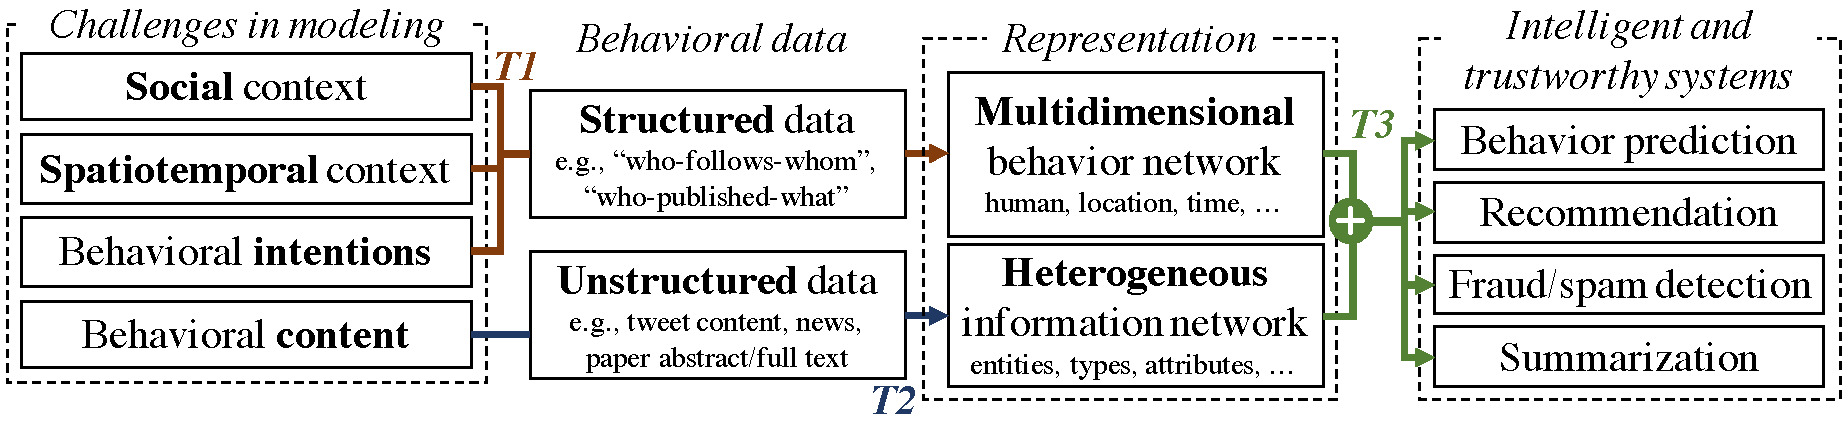
\includegraphics[width=0.65\textwidth]{figure/intro.pdf}
\vskip -0.18in
\caption{Towards building intelligent and trustworthy systems and addressing the four challenges, I have been proposing data-driven approaches of discovering rich knowledge from behavioral data by \textit{mining} behavior networks (T1), \textit{constructing} information networks (T2) and \textit{integrating} them into in-depth behavioral analysis (T3).}
\label{fig:intro}
\vskip -0.12in
\end{wrapfigure}

Behavior is defined as \textit{interaction} made by individuals in conjunction with themselves or their environment\footnote{Behavior -- Wikipedia, the free encyclopedia: \url{https://en.wikipedia.org/wiki/Behavior}}. Thanks to Information Technologies, the human behaviors are broadly recorded in an unprecedented level. This gives us an opportunity for getting insights of behaviors and our societies from large-scale real data. The Department of Defense (DoD) listed \textit{Computational Modeling of Human Behavior} as one of the six high-priority topics in DoD Basic Research\footnote{National Defense Industrial Association (NDIA) Conference Proceedings: \url{http://www.dtic.mil/ndia/}}. In order to provide a fundamental understanding and predictive capability of human behavior dynamics from individuals to societies, behavioral analysis has to face the following complexity of behavior: (1) human behaviors are highly dependent on \textit{social contexts}; (2) only by modeling \textit{spatiotemporal contexts}, can we understand when, where and how the behavior happens; (3) behavioral intentions including monetary incentives and other suspicious purposes are a nontrivial part of behavior modeling; (4) user preferences and sentiments on the \textit{unstructured content} are important driving factors. Experience-driven approaches rely on expertise in developing features of intelligent and trustworthy systems (e.g., recommender systems, anti-fraud/anti-spam systems). Taking the advantage of massive, available behavioral data, I have been proposing and promoting data-driven approaches that leverage the methodology of \textit{observation}, \textit{representation} and \textit{models} from real data beyond our eyes and hands. I focus on analyzing behavioral data with network models and algorithms relying little to none of human annotations for themes including (T1) mining multidimensional behavior networks with social spatiotemporal contexts, (T2) structuring behavioral content into heterogeneous information networks of entities and attributes, and (T3) integrating behavior networks and information networks for accuracy and interpretability.

\vskip 0.10in
\noindent {\large \bf I. THESIS AND POSTDOCTORAL WORK}
\vskip 0.01in

My thesis titled ``Modeling Complex Behaviors in Social Media'' focuses on Theme T1 of understanding behaviors under social spatiotemporal contexts, and my two-year postdoctoral research is broken down to T2 and T3 with contributions mostly to in-depth behavioral analysis with unstructured data. The three tasks form the full picture of ``Data-Driven Behavioral Analytics with Networks''.

\vskip 0.05in
\noindent {\large \bf T1. Mining behavior network with social spatiotemporal contexts}
\vskip 0.01in

During my five-year Ph.D., I feel fortunate joining the long-term collaboration between Tencent Weibo (one of the largest Twitter-style social platforms in China) and Tsinghua University, which keeps my hands on massive real data generated by millions of users and billions of social relations and real-world problems including building social recommender systems and anti-fraud systems. 

\vskip 0.03in
\noindent {\bf T1.1 Modeling social spatiotemporal contexts for behavior prediction}

%\cite{liu2010mining,liu2012mining,jiang2012socialcontextual,jiang2014scalable,jiang2012socialrecommendation,jiang2015social,jiang2016little,jiang2014fema,kuang2016steering,jiang2016catchingsocial}

\begin{wrapfigure}{R}{0.65\textwidth}
\vskip -0.12in
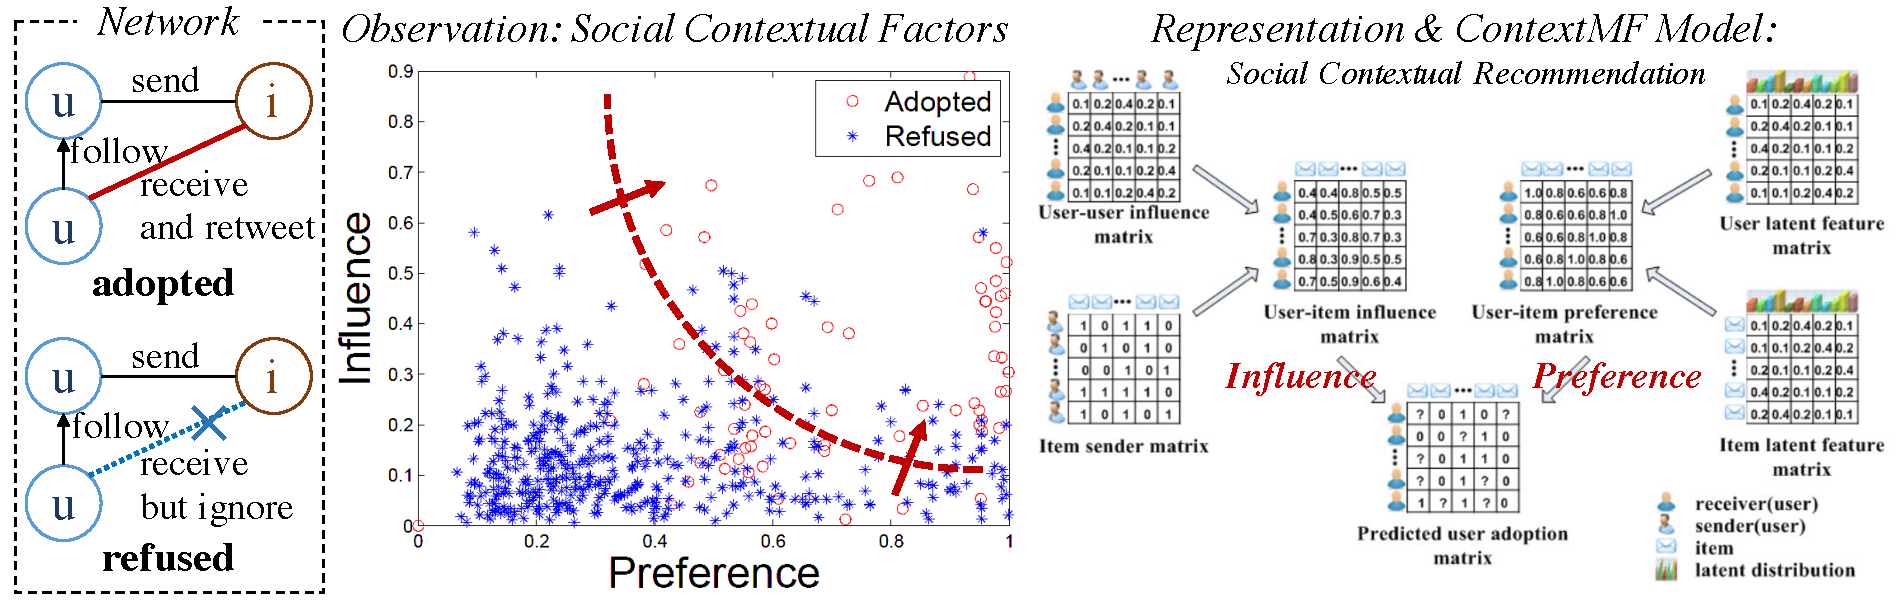
\includegraphics[width=0.65\textwidth]{figure/contextmf.pdf}
\vskip -0.18in
\caption{Uncovering two significant factors of user decisions with data, we proposed \textsc{ContextMF} \cite{jiang2012socialcontextual} that integrates preference and influence in social recommendation.}
\label{fig:contextmf}
\vskip -0.12in
\end{wrapfigure}

Weibo suffers from \textit{low} conversion rate: users received too much (less interesting) information from crowds and generated fewer than 6 retweets within every 100 news feed requests. Can we recommend tweets by predicting their behaviors to address the issue of information overload? Although collaborative filtering techniques have been widely used, we know little about why users adopt or reject items, which has been the bottleneck for further improving the recommending performance. How to fully exploit social contextual information from ``who-posts-what'' behavior network and ``who-follows-whom'' social network to reveal the information adoption mechanism, and accordingly propose a method for recommendation, is rather challenging and demanded.

To achieve this goal, we observe from the real network data that personal preference on the content and interpersonal influence from the sender are two significant factors that determine users' decisions (see Figure~\ref{fig:contextmf}). We propose a probabilistic matrix factorization model, \textsc{ContextMF} \cite{jiang2012socialcontextual}, to fuse the behaviors and social contexts. In this model, there are three low-rank latent spaces respectively corresponding to the user space, item space and influence space. They are regularized by the observed preference similarity matrix, content similarity matrix and interaction frequency matrix. The product of the user space and item space corresponds to the preference; the product of influence and preference is proportional to the probability of item adoption. Empirical results on two real social datasets (one from Weibo) demonstrate that \textsc{ContextMF} increases the accuracy of prediction by 21\% and 17\%, respectively.

\begin{wrapfigure}{R}{0.56\textwidth}
\vskip -0.07in
\begin{tabular}{cc}
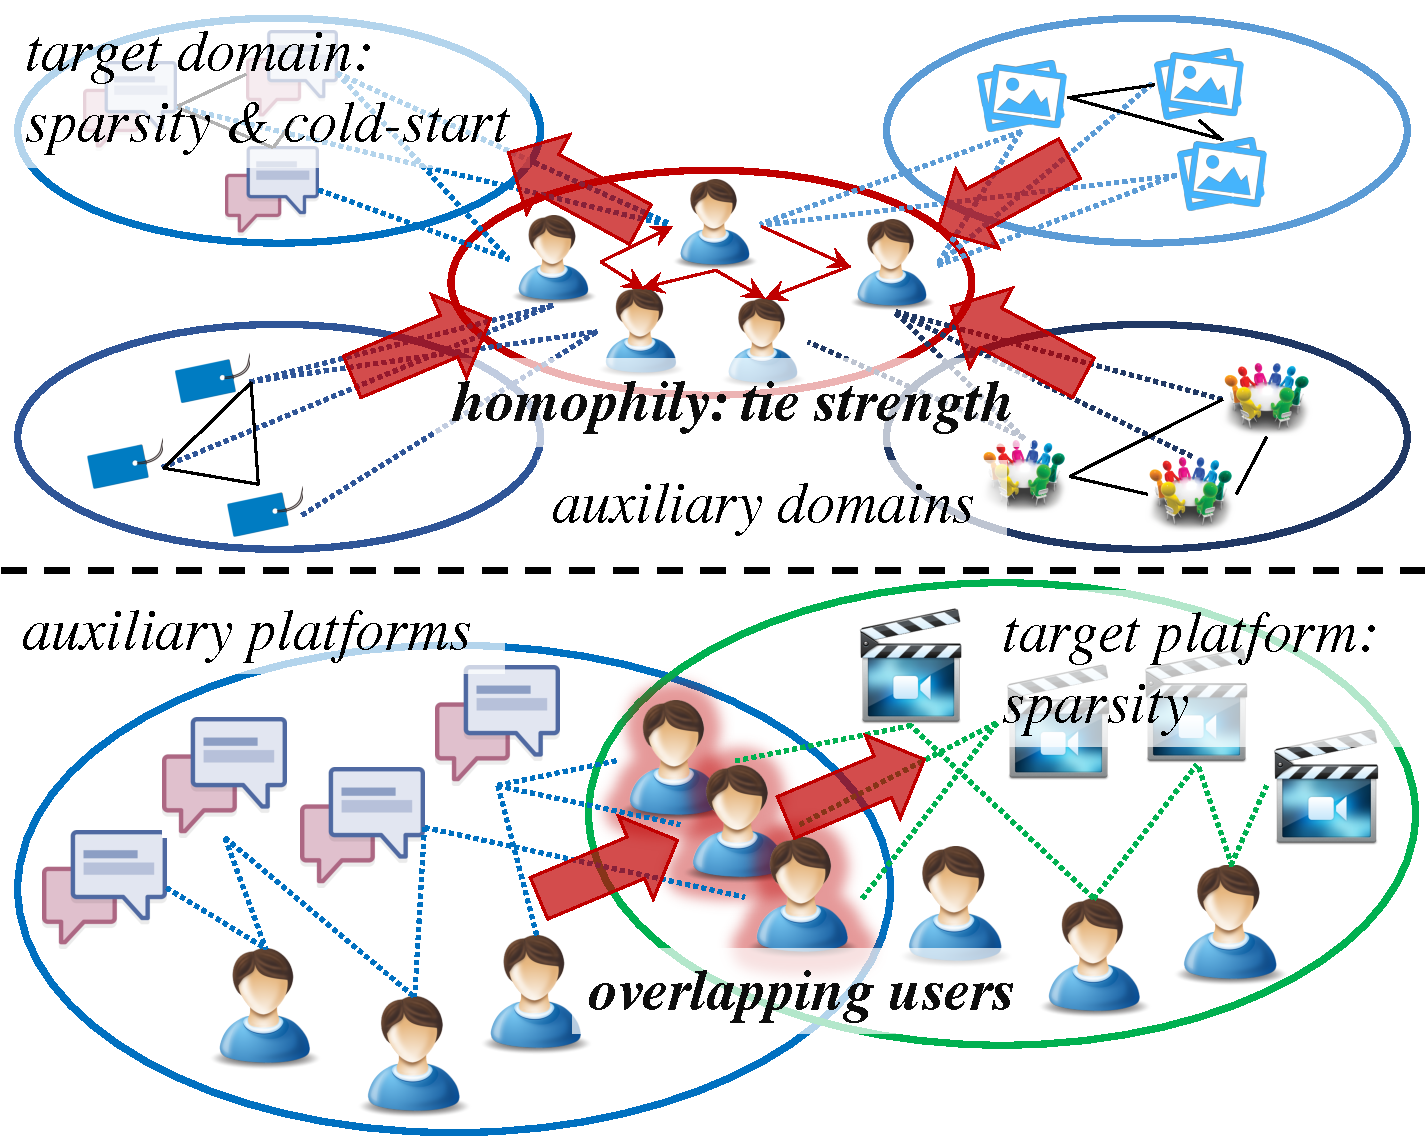
\includegraphics[width=0.27\textwidth]{figure/hybridrw-xptrans.pdf}
& 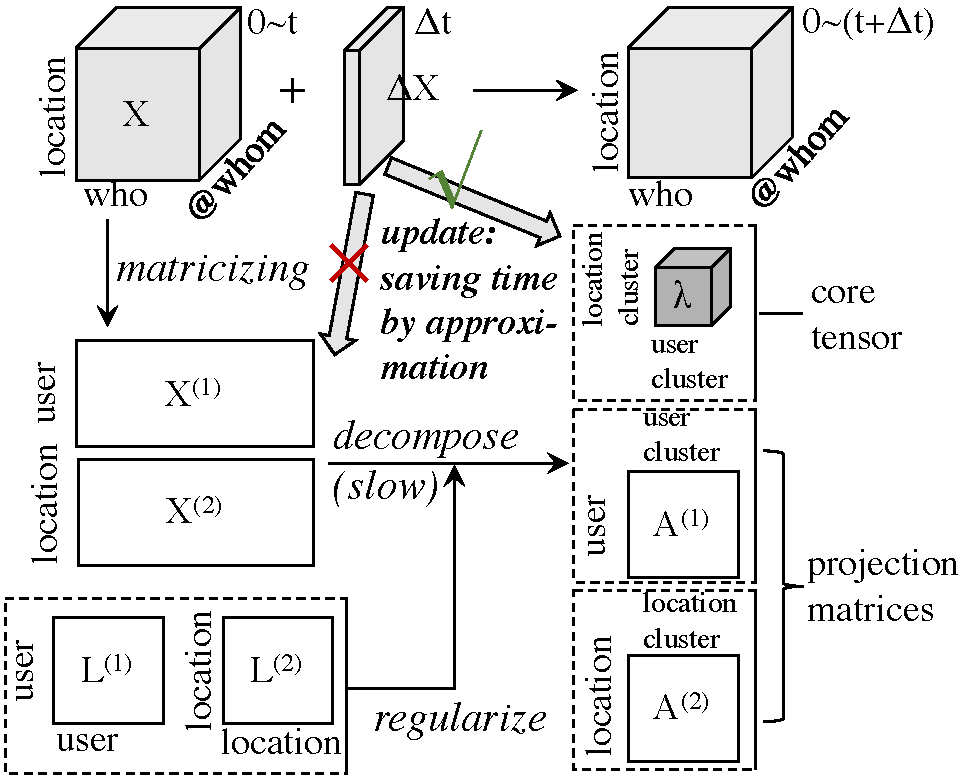
\includegraphics[width=0.27\textwidth]{figure/fema.pdf} \\
(a) \textsc{HybridRW} and \textsc{XPTrans}
& (b) \textsc{FEMA}
\end{tabular}
\vskip -0.12in
\caption{Contextual behavior modeling: (a) bridging behaviors across domains and platforms to alleviate the issue of sparsity, (b) modeling spatiotemporal information with Flexible Evolutionary Multifaceted Analysis.}
\label{fig:fema}
\vskip -0.12in
\end{wrapfigure}

\noindent {\em Cross-domain behavior modeling.} The principle is that if we have denser user-item links of behavioral data, we acquire more knowledge and thus predict more accurately. However, the real case comes to be sparsity and cold start (when the user has not yet adopted or rejected any item). Fortunately, the social platform enables users generating content in multiple domains such as profiling tags, images and interest groups. We propose Hybrid Random Walk (\textsc{HybridRW}) \cite{jiang2012socialrecommendation} to transfer knowledge across multiple domains on a star-structured network (see Figure~\ref{fig:fema}) for social recommendation. \textsc{HybridRW} collaboratively integrates multiple domains to discover the common knowledge of user tie strength in the central social domain and accordingly alleviates the sparsity issue in individual domains. Empirical results show that given profiling tag information, our method needs only 35\% training data of the target domain to achieve the same performance of taking all the training data but no profiling tag.

\noindent {\em Cross-platform behavior modeling.} A more important issue is that emerging platforms meet more serious sparsity and cold start problems. Can we utilize rich social platform data to improve the accuracy of predicting behaviors in other platforms (e.g., movie ratings in Netflix, ride requests in Uber)? The natural bridge across platforms is the small number of partially overlapping users, for example, users can register Uber with their Facebook accounts. How to make full use of the bridge is an open and challenging problem. We propose \textsc{XPTrans} \cite{jiang2016little} that transfers knowledge across platforms by jointly optimizing different user and item spaces on different platforms and using pairwise similarity of the overlapping users to constrain the spaces. By transferring via the little percentage (i.e., 1.1\%) of the overlapping users, the predicting performance on the non-overlapping users is even better than that on the overlapping users (who generate more data) without transfer.

\noindent {\em Spatiotemporal behavior modeling.} Human behavior is a product of and evolves with the changing of a multitude of interrelated factors such as physical environment, social identity and interaction. We represent behaviors of multiple dimensions of user who posts, user who is mentioned, word and location as high-order tensor sequences. We propose a Flexible Evolutionary Multi-faceted Analysis (\textsc{FEMA}) method \cite{jiang2014fema} based on a dynamic scheme of tensor factorization in which flexible regularizers of social-relationship and location-distance information are imposed to alleviate the high sparsity. To address the complexity issue, we give approximation algorithms based on Tensor Perturbation theory to factorize the updated tensor with sparse increments, where the loss bound is theoretically proved. Experimental results demonstrate that our method achieves 30.8\% higher accuracy when it considers multi-dimensions and 17.4\% higher accuracy when it uses the regularizers. Moreover, it can reduce the time cost from hours to minutes.

\noindent {\bf \underline{Impact.}}
\begin{compactitem}
\item \textsc{ContextMF} \cite{jiang2012socialcontextual} and \textsc{HybridRW} \cite{jiang2012socialrecommendation} are the $3^{rd}$ and $9^{th}$ most cited papers of CIKM 2012 with \textbf{121} and \textbf{47} citations among 146 accepted papers at the acceptance rate of 13.4\%, where as the median number of citations for CIKM 2012 is 11. Adding the feature of scalability, \textsc{ContextMF+} \cite{jiang2014scalable} has appeared in TKDE 2014 with \textbf{36} citations.
\item \textsc{ContextMF+} has been deployed in Weibo's recommender system. Online testing demonstrates that the conversion rate is improved from 5.78\% to 8.27\% (relatively \textbf{43\%}). Note that the rate is strongly related to the company's ad revenue.
\end{compactitem}

\vskip 0.03in
\noindent {\bf T1.2 Modeling social spatiotemporal contexts for suspicious behavior detection}

%\cite{jiang2014inferring,jiang2014detecting,jiang2014catchsync,jiang2015inferring,jiang2016catchingsynchronized,jiang2015general,jiang2016spotting,jiang2016suspicious}

\begin{wrapfigure}{R}{0.66\textwidth}
\vskip -0.12in
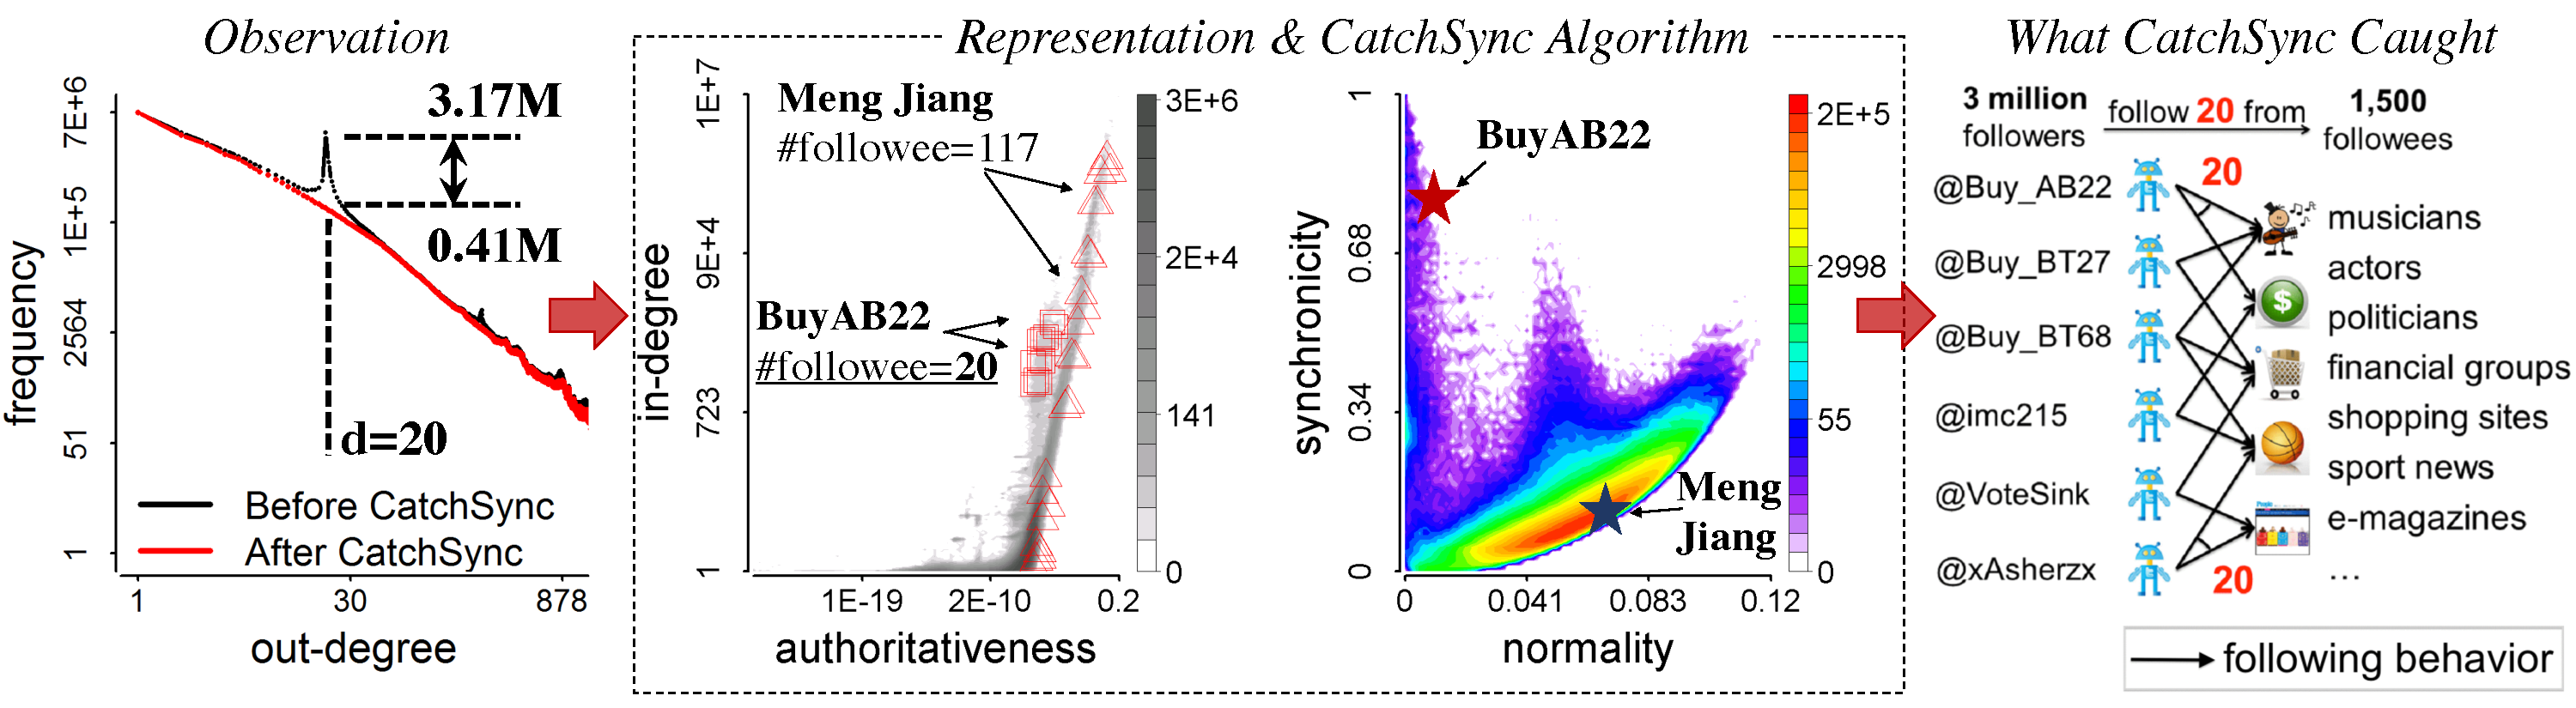
\includegraphics[width=0.66\textwidth]{figure/catchsync.pdf}
\vskip -0.18in
\caption{\textsc{CatchSync} \cite{jiang2014catchsync} spots that fake followers consistently connect to customers of similar features: their synchronized behaviors create spikes on degree distributions.}
\label{fig:catchsync}
\vskip -0.12in
\end{wrapfigure}

Given ``who-follows-whom'' networks, how can we automatically detect fake followers with high recall? The fraudsters are paid to make certain accounts seem more legitimate or famous through giving them many additional followers. Twitter admitted 5\% of its users are fake\footnote{Business Insider. \url{http://www.businessinsider.com/5-of-twitter-monthly-active-users-are-fake-2013-10}}; Weibo suffered the same and more serious problem. Experience-driven approaches learn classifiers with features such as the numbers of followees, hashtags and URLs. However, the fraudsters are smart: they don't have to follow or publish many; instead, a large set of them consistently connect to the customers.

Essentially, we reconsider the detection problem by revealing the fraudsters' manipulation on the network. As shown in Figure~\ref{fig:catchsync}, the spikes on the out-degree distribution indicate millions of anomalous nodes on the network. The fraudsters exhibit behavior that is (1) synchronized (i.e., cause to occur at the same rate): they often connect to the very same 20, 100 or 500 targets, and (2) abnormal: their behavior pattern is different from the majority of nodes. We propose a scalable and parameter-free algorithm, \textsc{CatchSync} \cite{jiang2014catchsync}, to measure the two properties (synchronicity and normality) of groups of followees. We prove that the synchronicity has a parabolic lower bound of the normality. \textsc{CatchSync} detects millions of fake followers who have unexpectedly high synchronicity and successfully recovers the distribution into a power-law shape, which demonstrates high recall of the performance.

\noindent {\em Evaluating suspiciousness across dimensions.} Besides inflating the number of fans, Weibo's fraudsters are trying to manipulate the popularity of trending topics. So which seems more suspicious: 5,000 tweets from 200 users on 5 IP addresses, or 10,000 tweets from 500 users on 500 IP addresses but all with the same hashtag and all in 10 minutes? The literature has many methods that find dense blocks in matrices and tensors, but no method gives a principled way to score the suspiciousness of dense blocks with different numbers of dimensions such as user, hashtag, location and time. To address this issue, we give axioms that any metric of suspiciousness should satisfy and propose an intuitive, principled metric that satisfies the axioms, and is fast to compute. We further propose \textsc{CrossSpot} \cite{jiang2015general} to spot suspicious regions and sort them in importance order. Empirical results show that \textsc{CrossSpot} improves the F1 score by 68\% when capturing hashtag-hijacking and retweet-boosting in Weibo datasets spanning 0.3 billion posts.

\noindent {\bf \underline{Impact.}}
\begin{compactitem}
\item \textsc{CatchSync} \cite{jiang2014catchsync} was selected as one of the best paper finalists of KDD 2014 with \textbf{39} citations. The algorithm has been taught in (1) CMU 15-826 ``Multimedia Databases and Data Mining'', (2) UMich EECS 598 ``Graph Mining and Exploration at Scale'', and (3) ASONAM 2016 Tutorial ``Identifying Malicious Actors on Social Media'' by Kumar et al. from UMCP.
\item \textsc{LockInfer} \cite{jiang2014inferring} was the first paper to introduce the concept of \textit{Camouflage} in fraud detection, and it now has \textbf{27} citations and it has appeared in KAIS 2015 \cite{jiang2015inferring}. \textsc{CrossSpot} \cite{jiang2015general} has \textbf{15} citations and it has appeared in TKDE 2016 \cite{jiang2016spotting}. The KDD 2016 best research paper by Hooi et al. cited all these three algorithms.
\item Our survey paper about current trends and future directions on suspicious behavior detection has appeared in IEEE Intelligent Systems (IS) \cite{jiang2016suspicious}. It was ranked as the top 10 most frequently downloaded documents in the IS from January to March 2016.
\end{compactitem}

\vskip 0.05in
\noindent {\large \bf T2. Structuring behavioral content into heterogeneous information network}
\vskip 0.01in

%\cite{gupta2014biperpedia,liu2015mining,ren2015clustype,jiang2016metapad}

\begin{wrapfigure}{R}{0.53\textwidth}
\vskip -0.18in
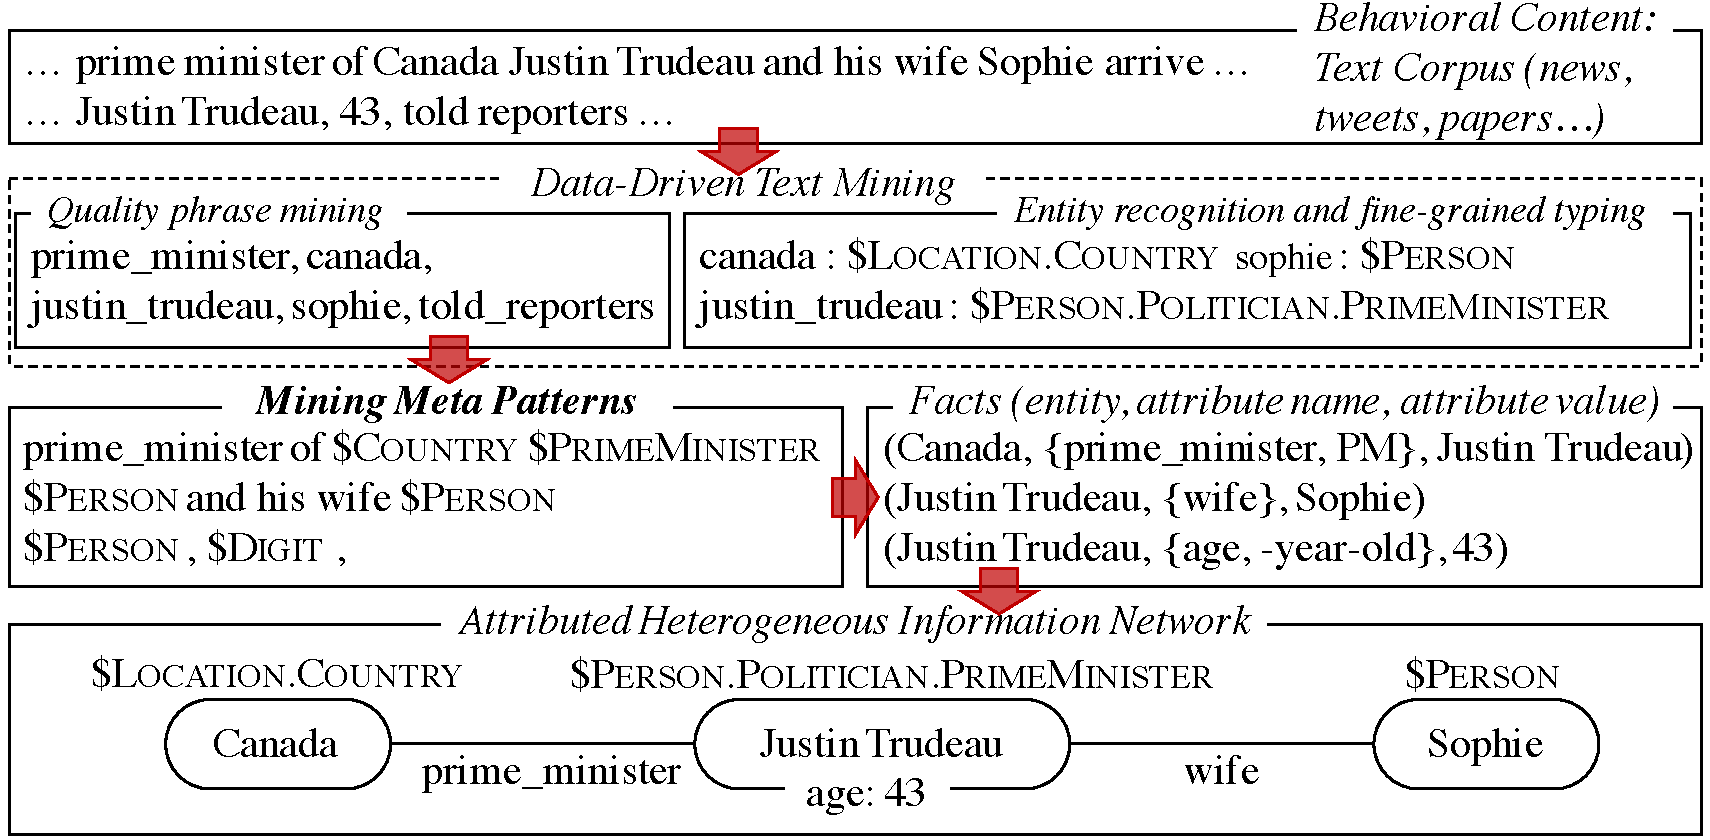
\includegraphics[width=0.53\textwidth]{figure/metapad.pdf}
\vskip -0.18in
\caption{Structuring text into heterogeneous information networks: \textsc{MetaPAD} jointly extracts \tuple{entity type}{attribute name}{value type} tuples and \tuple{entity}{attribute name}{attribute value} tuples for high precision and high recall. It is automated and domain-independent.}
\label{fig:metapad}
\vskip -0.12in
\end{wrapfigure}

In Theme T1, I work on modeling social spatiotemporal contexts in behavioral data: the contexts are naturally well-structured and thus can be represented as multidimensional behavior networks. However, the behavioral content, especially the text corpus in tweets and papers, is information-rich but \textit{unstructured}. Structuring the text into heterogeneous information networks will enables deep understanding of the behavioral content. Given the text data, e.g., a news corpus with sentence~\#1 in Figure~\ref{fig:metapad}, can we extract (1) the \pair{entity type}{attribute name} pair, e.g., \pair{\cscountry}{president} and (2) the \tuple{entity}{attribute name}{attribute value} tuple, e.g., \tuple{Burkina Faso}{president}{Blaise Compaor$\acute{e}$}?

Google mines users' fact-seeking queries (e.g., ``president of united states'') with \eapatterns ($E$ for entity and $A$ for attribute name) such as ``$A$ of $E$'' and ``$E$ 's $A$''. However, query-log word distributions are highly constrained compared with ordinary written language. Thus \eapatterns like ``$E$ $A$'' and ``$A$, $E$'' which lack attribute values may generate noisy attribute name extractions. The state-of-the-art open IE systems learn syntactic and lexical patterns of expressing relationships for extracting entity-level tuples. However, they may generate incorrect or imprecise extractions (e.g., \tuple{President Blaise Compaor$\acute{e}$}{have}{government of Burkina Faso} in which ``have'' is not a good attribute name for the entity by ignoring the type information).

Our idea is to investigate joint extraction of the type-level \tuple{entity type}{attribute name}{attribute value type} tuples (adding ``value type'' into the pair) and the entity-level tuples because these two extraction processes can mutually enhance each other. First, extracting a frequent type-level tuple is easier (due to its higher frequency) than extracting a concrete entity-level tuple. Second, the type distributions of the concrete entities indicate the appropriate level of the entity types in the type-level tuples. This joint extraction helps find the entity-level tuples with low counts to improve recall if the type-level tuples are frequent and attach attribute names to appropriate levels of types to improve precision. Based on this, we propose a novel methodology, \textit{Meta Pattern Mining}, that mines frequent and informative semantic patterns indicating type-level tuples, called \textit{meta patterns}. For sentence~\#3 in Figure~\ref{fig:metapad}, if we replace ``U.S.'' with \cscountry and replace ``Barack Obama'' with \cspolitician, and carefully segment the sentence, we can generate meta pattern ``\cscountry president \cspolitician'' and tuple \tuple{\cscountry}{president}{\cspolitician}. Taking the meta pattern back to the text, we can extract a set of entity-level tuples. It is worth noting that mining meta patterns allows \textit{automatic} and \textit{domain-independent} attribute discovery from massive corpora, relying on \textit{no} linguistic assumptions \textit{nor} query logs \textit{nor} human annotations.

Mining meta patterns has the advantages described above but it is challenging. First, imprecise boundaries of meta patterns may generate incorrect or incomplete extractions. Second, adjusting the level of entity types in a meta pattern is nontrivial. Third, it is necessary to group synonymous meta patterns. We develop a \underline{Meta} \underline{P}attern-driven \underline{A}ttribute \underline{D}iscovery (\textsc{MetaPAD}) framework, which first pre-processes text data to extract entities and their types as input in a data-driven and distantly-supervised manner and then mines the meta patterns with three new techniques to address the challenges for attribute discovery. Experiments on news, tweets and biomedical text data demonstrate that \textsc{MetaPAD} improves the F1 scores over the state-of-the-art by 32--51\% in \pair{entity type}{attribute name} extraction and by 26--35\% in \tuple{entity}{attribute name}{attribute value} extraction.

\noindent {\bf \underline{Impact.}}
\begin{compactitem}
\item \textsc{MetaPAD} was collaborated with Dr. Taylor Cassidy, Dr. Lance M. Kaplan and Dr. Timothy R. Hanratty from Army Research Lab \cite{jiang2016metapad}. The package is transferring to ARL in the Network Science Collaborative Technology Alliance (NS CTA) project. 
\end{compactitem}

\vskip 0.05in
\noindent {\large \bf T3. Integrating behavior network and information network for behavior summarization}
\vskip 0.01in

%\cite{jiang2016catchtartan,gui2016large}

\begin{wrapfigure}{R}{0.3\textwidth}
\vskip -0.18in
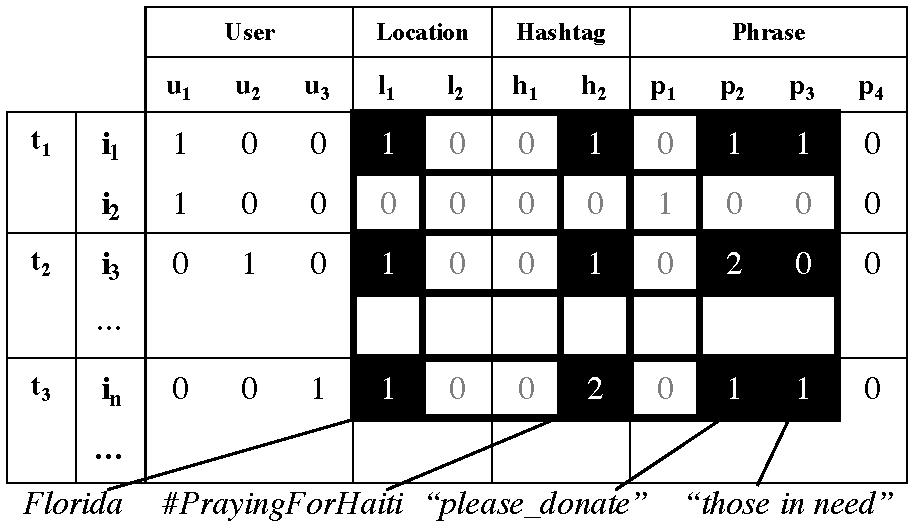
\includegraphics[width=0.3\textwidth]{figure/catchtartan.pdf}
\vskip -0.18in
\caption{Each row is a tweet. \cite{jiang2016catchtartan} detects and summaries events by looking for \textit{Tartans} in ``two-level matrix'' which represents every dimension of tweets including time, location and \textit{phrase}.}
\label{fig:catchtartan}
\vskip -0.20in
\end{wrapfigure}

Fusing structured and unstructured data of human behaviors is substantial for in-depth behavioral analysis. Even bringing the quality phrases that were extracted from the unstructured content into behavior modeling has already been valuable and challenging. For example, given phrases and spatiotemporal contexts of tweets, can we automatically detect and summarize events from the multidimensional data? High-order tensor assumes that every behavior has exactly one value in every dimension, for example, a tweet has one user, one phrase and one hashtag. However, the real case is a behavior may have multiple values in a dimension. We propose ``two-level matrix'' that enables representing every single tweet: (1) the first/second level of columns are dimensions/dimensional values, (2) the first/second level of rows are time slices/behaviors. Thus, an event summary can be defined as a set of interesting dimensions and consecutive time slices, a set of interesting values in each selected dimension and a set of behaviors (tweets) in each selected slice, which forms a ``Tartan'' in the matrix (see Figure~\ref{fig:catchtartan}). We develop a propagation method \textsc{CatchTartan} \cite{jiang2016catchtartan} to capture the Tartans in a principled and scalable way: it determines the meaningfulness of every operation of updating the Tartan with the Minimum Description Length (MDL) principle. Empirical results show that it outperforms the tensor-based approaches, requires no parameter and provides comprehensive summaries of local events in tweets and research trends in academic data.

\noindent {\bf \underline{Fun facts.}}
\begin{compactitem}
\item ``Tartan'' is the team nickname of CMU: Women's and men's, football and baseball, swimming and tennis.
\item \textsc{CatchTartan} \cite{jiang2016catchtartan} was accepted as full paper in KDD 2016 (70 from 784 submissions; 8.9\%). It is the $1^{st}$ conference paper that Dr. Han (UIUC) and Dr. Faloutsos (CMU) co-authored, though they have been predicted to be co-authors for long.
\item This is the \underline{$9^{th}$} paper I have collaborated with Dr. Faloutsos as the $1^{st}$ author after my \underline{$9$}-month visit in CMU.
\end{compactitem}

\vskip 0.10in
\noindent {\large \bf II. FUTURE RESEARCH DIRECTIONS}
\vskip 0.01in

When more real-world applications (e.g., economics, politics, business intelligence) are incorporating data science, the data-driven behavioral analytics should also be incorporating with other field sciences (e.g., behavioral science, psychological science, social science). The need for intelligence, trustworthiness and scalability in user-oriented systems will only increase.

\vskip 0.08in
\noindent {\large \bf Mid-Term Research Plan }
\vskip 0.01in

With respect to my shorter term plan (first 3-5 years), I provide a more detailed outline of the thrusts and challenges that I am planning to tackle, both contributing to the data-driven framework of behavioral analysis that support decision-making processes.

\vskip 0.02in
\noindent {\bf D1. Intelligence: Integrating structured and unstructured data for in-depth behavioral analysis}
\vskip 0.01in

\noindent {\em 1. Integrating information networks from behavioral content for contextual behavior modeling.}
In my thesis and postdoctoral research, I have improved the state-of-the-art in modeling user behavior with structured data: predicting behaviors with contexts and catching suspicious behaviors. However, if we don't model the content with structures, big data means big mess. Fortunately, the data-driven meta pattern mining approaches shed light on automatically structuring the content into a rich network of entities and attributes. How to grab this opportunity to develop accurate and interpretable predictive models needs to be investigated.

\noindent {\em 2. Predicting behavioral contexts over predicting contextual behaviors.}
Suppose we are able to predict with 100\% accuracy if a behavior will happen given full contexts of it. Then given a subset of the contexts, can we predict the set of the rest contexts? For example, if one wants to solve the fraud detection problem on Weibo, which experts, papers and algorithms he/she should find, read and try? Assume that we have represented the applications, datasets and other entities as nodes in an $n$-node heterogeneous network, the complexity of searching for the optimum is too high: the space of solutions is $O(n!)$. How to reduce the complexity into a practical level by pruning impossible permutations with insights from behavioral and psychological sciences is interesting and challenging.

\vskip 0.02in
\noindent {\bf D2. Trustworthiness: Structuring reliable information networks from behavioral content}
\vskip 0.01in

Our meta-pattern mining is a general, data-driven methodology to be used across multiple NLP tasks such as entity recognition and typing, attribute/relationship extraction and slot filling in an automated way. However, a portion of the extractions may still be incorrect or imprecise, for example, the text ``McDonald's U.S. President...'' may mistake a McDonald executive as a U.S. president. In order to structure reliable information from behavioral content, it is necessary to enhance mining results with majority voting-based conflict resolution, sentence structure-based entity refinement and conditional functional dependency rule mining.

\vskip 0.02in
\noindent {\em \large Collaborative research.} I am eager for collaborations with experts of Natural Language Processing, Text Mining, Machine Learning, Artificial Intelligence and Cyber-Physical Security and Systems, towards the ultimate goal of building efficient systems of intelligence and trustworthiness for human beings and our society.

\vskip 0.03in
\noindent {\large \bf Long-Term Vision: Interdisciplinary Research and Real-World Impact of Behavioral Analytics}
\vskip 0.01in

The future of behavioral analytics locates at collaboration between data scientists and behavioral psychologists, which is a formidable combination that could not be accomplished without pooling these unique skills that differ by scientific training.

\noindent {\em 1. Bringing psychological expertise into data technology.} 
Data in itself is nothing. We can only create value if we turn it into information. Data expertise alone is not sufficient to truly understand human behaviors. Behavioral scientists know more about the human brain. They are specialized in cognitive psychology. How do people perceive? How do they reach a decision? This kind of knowledge is crucial if we want to intervene users' behavior. Take the social contextual recommendation as an example. When I was struggling in understanding how Weibo users decide to forward or ignore a message, a Science paper \cite{salganik2006experimental} emerged to help. Salganick et al. adopted an experimental approach to the study of social influence in cultural markets, inspired by which I reconsidered the information adoption mechanism of Weibo and proposed that preference and influence were two major contextual factors. Experiments on real large data demonstrated my assumption (see Figure~\ref{fig:contextmf}) and the proposed model \textsc{ContextMF} significantly improved Weibo's recommender systems. It is important to realize that vision if we bring real psychological expertise into our data science.

\noindent {\em 2. Facilitating psychological discovery processes with data science.}
Data-driven approaches have enormous potential to change the way psychological scientists observe human behavior. Big data leads researchers to a point where they can collect behavioral information without sampling human participants at all. Social media, e.g., Facebook, Twitter, are the new ``macroscopes of human behavior''. Technology such as smart phones and wearable sensors can gather information on physical activity, social interactions, and so on. This offers us a clue to understanding basic psychological principles and behavioral theories for experimentation. Psychological scientists and data scientists have a vested interest in working together to yield more explanatory insight that can change the world.

\noindent {\em 3. Deploying scalable behavior modeling for real systems.}
To scale complex behavior models to the high volume of data, my research efficiently exploits the structure of multidimensional behavior networks and heterogeneous information networks. It is significantly valuable to deploy evolutionary analysis (e.g., \cite{jiang2014scalable,jiang2014fema}) and scalable algorithms (e.g., \cite{jiang2014catchsync,jiang2016catchtartan}) across a wide variety of applications.

\vskip 0.02in
\noindent {\em \large Contributing to the community.} I am focused on studying and promoting Data-Driven Behavioral Analytics. I have given two 3-hour tutorials in major conferences (i.e., ICDM 2015 \cite{jiang2015behavior} and CIKM 2016 \cite{jiang2016data}). Each had 50+ audience, and we won the honorium for both. I also have written two book chapters about user behavior modeling \cite{jiang2016mining,jiang2016behavior}.

\vskip 0.02in
\noindent {\em \large Funding opportunities.} First, based on the idea of \textsc{CatchTartan} \cite{jiang2016catchtartan}, I contributed significantly to the technical content in the proposal ``NSF III: Small: Multi-Dimensional Structuring, Summarizing and Mining of Social Media Data''. It has been awarded to the PI Dr. Jiawei Han by NSF IIS (08-01-2016 to 07-31-2019, \$500,000). I am the major supported member\footnote{NSF IIS 16-18481. \url{http://hanj.cs.illinois.edu/projs/social\_media.htm}}. Besides ``Information Integration and Informatics'' (III), ``Secure and Trustworthy Cyberspace'' (SaTC) also encourages the study of behavior analysis. Second, I have extensively collaborated with U.S. Army Research Lab (ALC and APG) in the NS CTA projects. Third, I have international relations with China's institutes (e.g., Tsinghua, Microsoft Research Asia) and IT companies (e.g., Tencent, Alibaba).

\vspace{-0.20in}
\small{
\begin{footnotesize}
\bibliographystyle{unsrt}
\bibliography{research_statement_jiang}
\end{footnotesize}
}

\end{document}


